\documentclass[table]{beamer}
%[]中可以使用draft、handout、screen、transparency、trancompress、compress等参数

%指定beamer的模式与主题
\mode<presentation>
{
  \usetheme{Madrid}
%\usetheme{Boadilla}
%\usecolortheme{default}
%\usecolortheme{orchid}
%\usecolortheme{whale}
%\usefonttheme{professionalfonts}
}

%\usetheme{Madrid}
%这里还可以选择别的主题:Bergen, Boadilla, Madrid, AnnArbor, CambridgeUS, Pittsburgh, Rochester, Warsaw, ...
%有导航栏的Antibes, JuanLesPins, Montpellier, ...
%有内容的Berkeley, PaloAlto, Goettingen, Marburg, Hannover, ...
%有最小导航栏的Berlin, Ilmenau, Dresden, Darmstadt, Frankfurt, Singapore, Szeged, ...
%有章和节表单的Copenhagen, Luebeck, Malmoe, Warsaw, ...

%\usecolortheme{default}
%设置内部颜色主题(这些主题一般改变block里的颜色);这个主题一般选择动物来命名
%这里还可以选择别的颜色主题,如默认的和有特别目的的颜色主题default,structure,sidebartab,全颜色主题albatross,beetle,crane,dove,fly,seagull,wolverine,beaver

%\usecolortheme{orchid}
%设置外部颜色主题(这些主题一般改变title里的颜色);这个主题一般选择植物来命名
%这里还可以选择别的颜色主题,如默认的和有特别目的的颜色主题lily,orchid,rose

%\usecolortheme{whale}
%设置字体主题;这个主题一般选择海洋动物来命名
%这里还可以选择别的颜色主题,如默认的和有特别目的的颜色主题whale,seahorse,dolphin

%\usefonttheme{professionalfonts}
%类似的还可以定义structurebold,structuresmallcapsserif,professionalfonts

% 控制 beamer 的风格,可以根据自己的爱好修改
%\usepackage{beamerthemesplit} %使用 split 风格
%\usepackage{beamerthemeshadow} %使用 shadow 风格
%\usepackage[width=2cm,dark,tab]{beamerthemesidebar}

%插入音标
%\usepackage{tipa}
%\AtBeginDocument{
  %\renewcommand\textipa{\fontencoding{T3}\selectfont}
%}
%\AtBeginDocument{
  %\renewcommand\textipa[2][r]{{\fontfamily{cm#1}\tipaencoding #2}}
%}
%\renewenvironment{IPA}[1][r]
 %{\fontfamily{cm#1}\tipaencoding}
 %{}

% 设定英文字体
%\usepackage{fontspec}
% Fix bugs for fontspec in TeXLive2015
\ifdefined\suppressfontnotfounderror
  \expandafter\let\csname xetex_suppressfontnotfounderror:D\endcsname
    \suppressfontnotfounderror
\else
  \expandafter\let\csname xetex_suppressfontnotfounderror:D\endcsname
    \luatexsuppressfontnotfounderror
\fi
\usepackage[no-math]{fontspec}
\setmainfont{Times New Roman}
\setsansfont{Arial}
\setmonofont{Courier New}

% 设定中文字体
\usepackage[BoldFont,SlantFont,CJKchecksingle,CJKnumber]{xeCJK}
%\setCJKmainfont[BoldFont={Adobe Heiti Std},ItalicFont={Adobe Kaiti Std}]{Adobe Song Std}
\setCJKmainfont[BoldFont={Adobe Heiti Std},ItalicFont={Adobe Kaiti Std}]{WenQuanYi Micro Hei}
\setCJKsansfont{Adobe Heiti Std}
\setCJKmonofont{Adobe Fangsong Std}
\punctstyle{hangmobanjiao}

\defaultfontfeatures{Mapping=tex-text}
\usepackage{xunicode}
\usepackage{xltxtra}

\XeTeXlinebreaklocale "zh"
\XeTeXlinebreakskip = 0pt plus 1pt minus 0.1pt

\usepackage{setspace}
\usepackage{colortbl,xcolor}
\usepackage{hyperref}
%\hypersetup{xetex,bookmarksnumbered=true,bookmarksopen=true,pdfborder=1,breaklinks,colorlinks,linkcolor=blue,filecolor=black,urlcolor=cyan,citecolor=green}
\hypersetup{xetex,bookmarksnumbered=true,bookmarksopen=true,pdfborder=1,breaklinks,colorlinks,linkcolor=cyan,filecolor=black,urlcolor=blue,citecolor=green}

% 插入图片
\usepackage{graphicx}
\graphicspath{{figures/}}
% 图文混排
%\usepackage{picins}
\usepackage{floatflt}

% 可能用到的包
\usepackage{amsmath,amssymb}
%插入多媒体
%\usepackage{media9}
%\usepackage{movie15}
\usepackage{multimedia}
\usepackage{multicol}
\usepackage{multirow}

% 定义一些自选的模板,包括背景、图标、导航条和页脚等,修改要慎重
% 设置背景渐变由10%的红变成10%的结构颜色
%\beamertemplateshadingbackground{red!10}{structure!10}
%\beamertemplatesolidbackgroundcolor{white!90!blue}
% 使所有隐藏的文本完全透明、动态,而且动态的范围很小
\beamertemplatetransparentcovereddynamic
% 使itemize环境中变成小球,这是一种视觉效果
\beamertemplateballitem
% 为所有已编号的部分设置一个章节目录,并且编号显示成小球
\beamertemplatenumberedballsectiontoc
% 将每一页的要素的要素名设成加粗字体
\beamertemplateboldpartpage

% item逐步显示时,使已经出现的item、正在显示的item、将要出现的item呈现不同颜色
\def\hilite<#1>{
 \temporal<#1>{\color{gray}}{\color{blue}}
    {\color{blue!25}}
}

\renewcommand{\today}{\number\year 年 \number\month 月 \number\day 日}

%五角星
\usepackage{MnSymbol}

%去除图表标题中的figure等
\usepackage{caption}
\captionsetup{labelformat=empty,labelsep=none}

\usepackage{tabu}
\usepackage{multirow}
%表格自动换行
\usepackage{tabularx} 

% 千分号
%\usepackage{textcomp}

%罗马数字
\makeatletter
\newcommand{\rmnum}[1]{\romannumeral #1}
\newcommand{\Rmnum}[1]{\expandafter\@slowromancap\romannumeral #1@}
\makeatother

%分栏
\usepackage{multicol}

%\usepackage{enumitem}
%\usepackage{enumerate}

%键盘
\usepackage{keystroke}

%心形
%\usepackage{fdsymbol}

%插入源代码
\usepackage{listings}
\lstset{
  language=perl,                  % 程序语言名称:TeX, Perl, R, sh, bash, Awk
  basicstyle=\normalsize\tt,      %\tt指monospace字体族,程序源代码使用此族字体表示更加美观
  numbers=left,                   % 行号位置(左侧)
  numberstyle=\small,             % 行号字体的字号
  stepnumber=1,                   % 行号的显示步长
  numbersep=5pt,                  % 行号与代码间距
  backgroundcolor=\color{white},  % 背景色;需要 \usepackage{color}
  showspaces=false,               % 不显示空格
  showstringspaces=false,         % 不显示代码字符串中的空格标记
  showtabs=false,                 % 不显示 TAB
  tabsize=4, 
  frame=shadowbox,                % 把代码用带有阴影的框圈起来
  captionpos=b,                   % 标题位置
  breaklines=true,                % 对过长的代码自动断行
  breakatwhitespace=false,        % 断行只在空格处
  extendedchars=false,            % 解决代码跨页时,章节标题,页眉等汉字不显示的问题
  %escapeinside={\%*}{*},         % 跳脱字符,添加注释,暂时离开 listings 
  %escapeinside=``,
  commentstyle=\color{red!50!green!50!blue!50}\tt,  %浅灰色的注释
  rulesepcolor=\color{red!20!green!20!blue!20},     %代码块边框为淡青色
  keywordstyle=\color{blue!70}\bfseries\tt,         %代码关键字的颜色为蓝色,粗体
  identifierstyle=\tt,
  stringstyle=\tt,                % 代码字符串的特殊格式
  keepspaces=true,
  breakindent=1em,
  %breakindent=22pt,
  %breakindent=4em,
  breakautoindent=true,
  flexiblecolumns=true,
  aboveskip=1em,                  %代码块边框
  xleftmargin=2em,
  xrightmargin=2em
}

%\setbeamercolor{alerted text}{fg=magenta}
\setbeamercolor{bgcolor}{fg=yellow,bg=cyan}
%\setbeamercolor{itemize/enumerate body}{fg=green}

\begin{document}

%\includeonlyframes{current}

\logo{
\includegraphics[height=0.08\textwidth]{qr.png}}

% 在每个Section前都会加入的Frame
\AtBeginSection[]
{
  \begin{frame}<beamer>
    %\frametitle{Outline}
    \frametitle{教学提纲}
    \setcounter{tocdepth}{3}
    \begin{multicols}{2}
      \tableofcontents[currentsection,currentsubsection]
      %\tableofcontents[currentsection]
    \end{multicols}
  \end{frame}
}
% 在每个Subsection前都会加入的Frame
\AtBeginSubsection[]
{
  \begin{frame}<beamer>
%%\begin{frame}<handout:0>
%% handout:0 表示只在手稿中出现
    \frametitle{教学提纲}
    \setcounter{tocdepth}{3}
    \begin{multicols}{2}
    \tableofcontents[currentsection,currentsubsection]
    \end{multicols}
%% 显示在目录中加亮的当前章节
  \end{frame}
}

% 为当前幻灯片设置背景
%{
%\usebackgroundtemplate{
%\vbox to \paperheight{\vfil\hbox to
%\paperwidth{\hfil\includegraphics[width=2in]{tijmu_charcoal.png}\hfil}\vfil}
%}
\begin{frame}[plain]
  \begin{center}
    {\Huge 故事中的统计学\\}
    \vspace{1cm}
    {\LARGE 天津医科大学\\}
    %\vspace{0.2cm}
    {\LARGE 生物医学工程与技术学院\\}
    \vspace{1cm}
    {\large 2017-2018学年下学期(春)\\ 公共选修课}
  \end{center}
\end{frame}
%}



%\includeonlyframes{current}

\title[平均数]{第二章\quad 精心挑选的平均数}
\author[Yixf]{伊现富(Yi Xianfu)}
\institute[TIJMU]{天津医科大学(TIJMU)\\ 生物医学工程与技术学院}
\date{2018年3月}

\begin{frame}
  \titlepage
\end{frame}

\begin{frame}[plain,label=current]
  \frametitle{教学提纲}
  \setcounter{tocdepth}{3}
  \begin{multicols}{2}
    \tableofcontents
  \end{multicols}
\end{frame}


\section{平均数}
\begin{frame}
  \frametitle{平均数 | 简介}
  \begin{block}{平均数}
把大量的数据压缩成一个单独的数字,这种做法在实践过程中轻而易举就可以实现。可惜这对于许多事情来说太过分了,模糊了事实上存在的巨大差异,掩盖了一些事情的真相。
  \end{block}
  \pause
  \begin{block}{笑话}
两个男人坐在一间酒馆里,其中一个人吃了一条牛腿,另一个人喝了两大桶啤酒。从统计学角度来看,每个人都喝了一桶啤酒,吃了半条牛腿,但实际的结果是,一个人吃得太多了,而另一个人却喝得烂醉。
  \end{block}
\end{frame}

\begin{frame}
  \frametitle{平均数 | 简介}
  \begin{block}{实例}
如果在一个村庄上有10个农民,其中1个农民拥有40头牛,其他9个农民一头牛也没有。如果计算他们的平均数,则每个农民拥有4头牛。对于9个一无所有的农民来说,这种平均的结果只是一个苍白无力的安慰、水中捞月的梦想。
  \end{block}
  \pause
  \begin{block}{实例}
    英国的普利茅斯市和美国的明尼阿波利斯市拥有同样的年平均气温——13$^{\circ}$C。而真实的气候:
    \pause
    \begin{itemize}
      \item 普利茅斯市:最冷的2月份最低气温也永远是8$^{\circ}$C,最热的7月份最高气温也绝对不会超过21$^{\circ}$C。
      \item 明尼阿波利斯市:在1月份平均气温通常都在-15$^{\circ}$C,到了夏天平均气温在30$^{\circ}$C以上,有时甚至会超过40$^{\circ}$C。
    \end{itemize}
  \end{block}
\end{frame}

\begin{frame}
  \frametitle{平均数 | 简介}
  \begin{block}{现象}
    当一个家伙希望用数据影响公众观点,或者向其他人推销广告版面,平均数便是一个经常被使用的伎俩,虽然偶尔是出于无心,但更多的时候是明知故犯。
  \end{block}
  \pause
  \begin{block}{原因}
    \begin{itemize}
      \item “平均数”这个词具有宽泛的涵义,不同情境下使用不同的平均数。
      \item 某种条件下,各种类型平均数的数值十分接近,如果出于一般的目的,便没有必要区分它们。
    \end{itemize}
  \end{block}
  \pause
  \begin{block}{\alert{结论}}
    当你被告知某个数是平均数时,除非能说出它的具体种类——均值、中位数还是众数,否则你对它的具体涵义仍知之甚少。
  \end{block}
\end{frame}

\begin{frame}
  \frametitle{平均数 | 种类}
  \begin{figure}
    \centering
    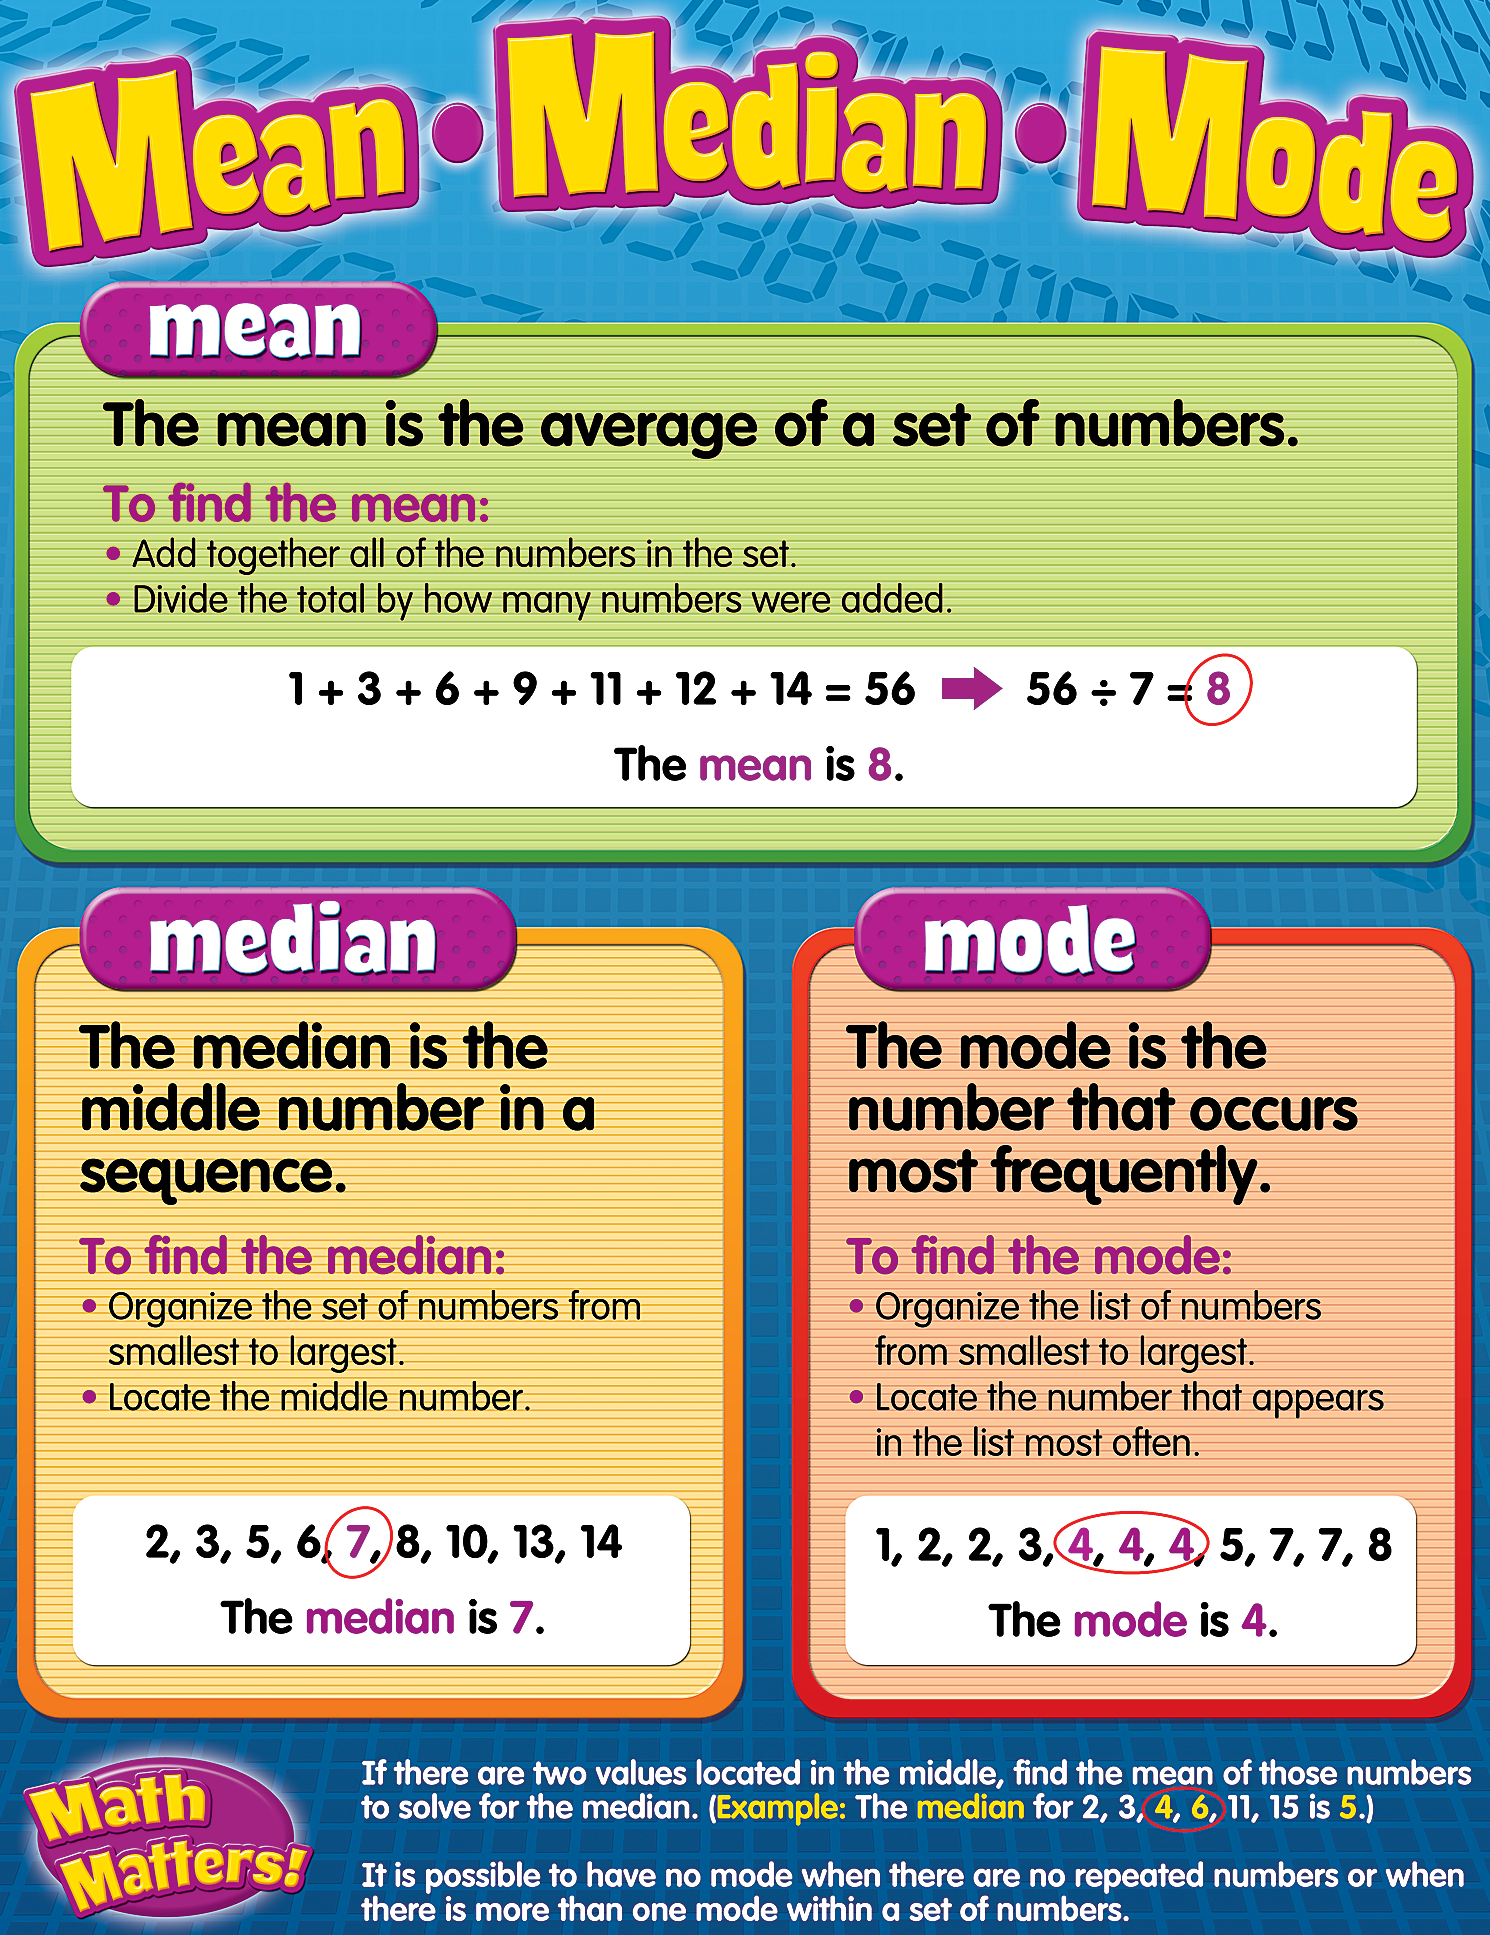
\includegraphics[width=0.5\textwidth]{c2.mmm.01.png}
  \end{figure}
\end{frame}

\begin{frame}
  \frametitle{平均数 | 种类}
  \begin{figure}
    \centering
    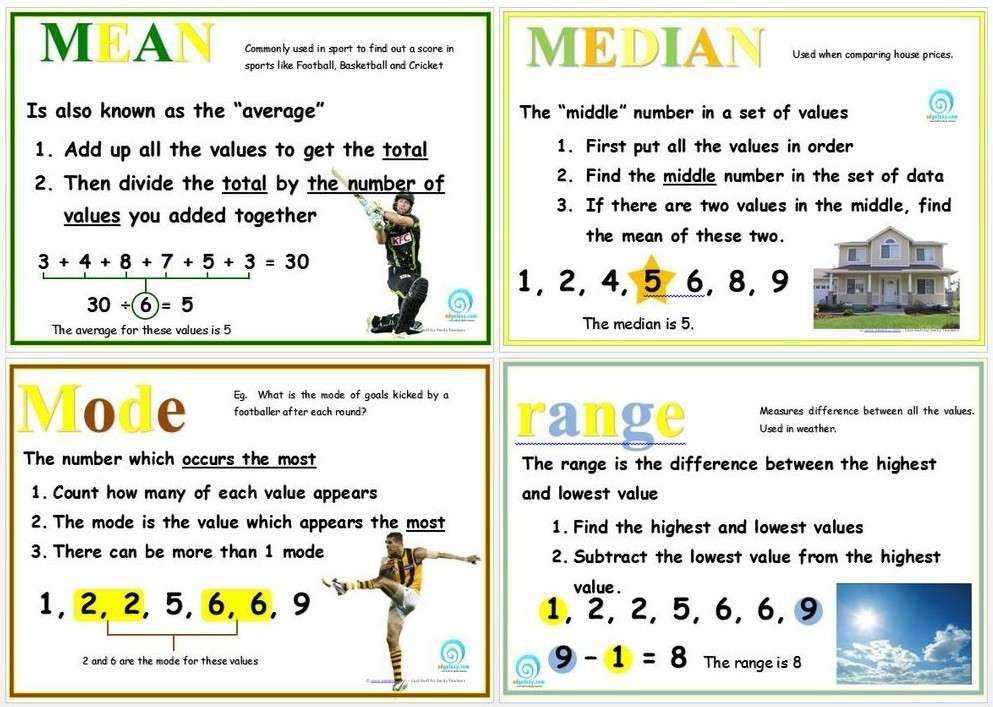
\includegraphics[width=0.9\textwidth]{c2.mmm.02.jpg}
  \end{figure}
\end{frame}

\begin{frame}
  \frametitle{平均数 | 种类}
  \begin{figure}
    \centering
    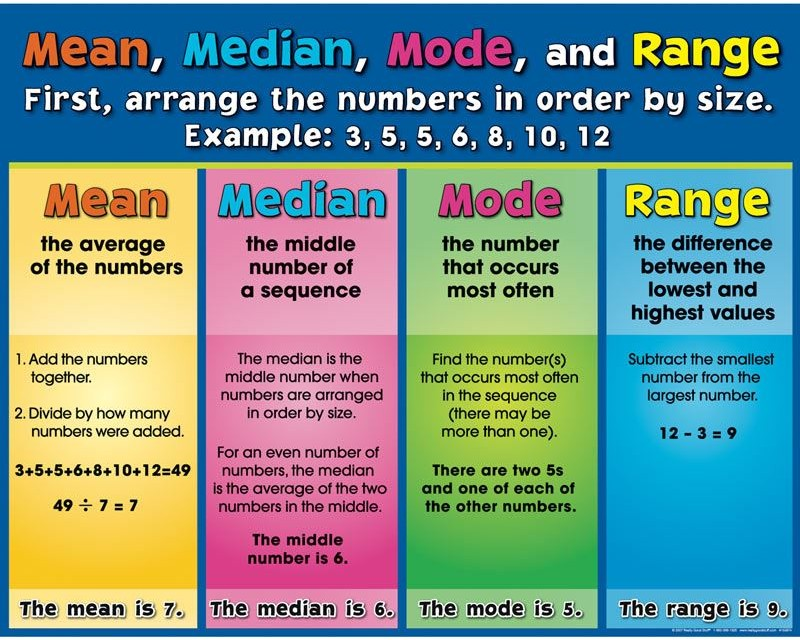
\includegraphics[width=0.8\textwidth]{c2.mmm.03.jpg}
  \end{figure}
\end{frame}

\begin{frame}
  \frametitle{平均数 | 百分位数}
  \begin{figure}
    \centering
    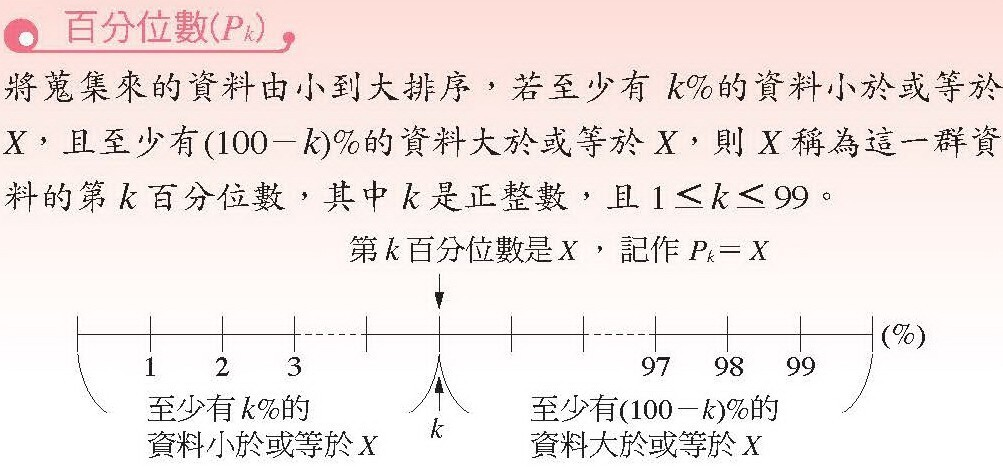
\includegraphics[width=0.65\textwidth]{c2.percentile.01.jpg}
    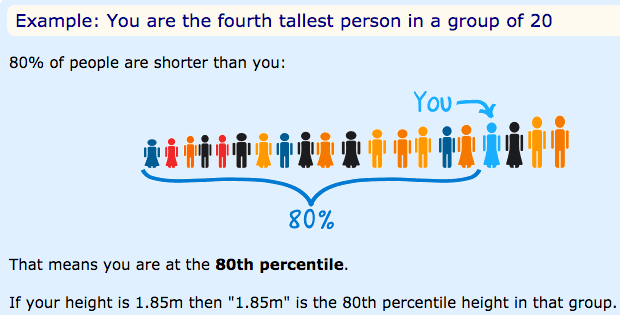
\includegraphics[width=0.65\textwidth]{c2.percentile.02.png}
  \end{figure}
\end{frame}

\begin{frame}
  \frametitle{平均数 | 四分位数}
  \begin{figure}
    \centering
    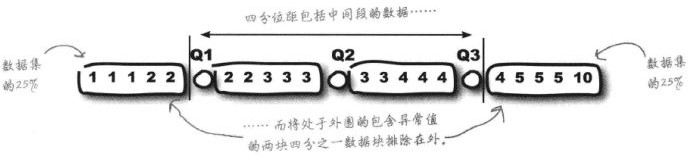
\includegraphics[width=0.8\textwidth]{c2.percentile.03.jpg}
    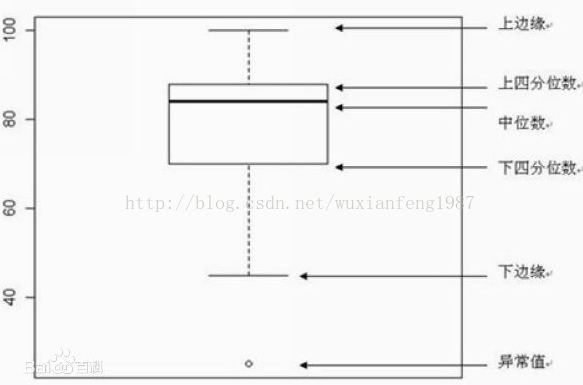
\includegraphics[width=0.6\textwidth]{c2.percentile.04.png}
  \end{figure}
\end{frame}

\section{花言巧语的收入}
\begin{frame}
  \frametitle{案例 | 小区居民年收入}
  \begin{block}{谁在说谎?}
    \begin{description}
      \item[房产中介] 小区居民平均年收入10000英镑
      \item[小区居民(纳税人)] 小区居民平均年收入只有2000英镑
      \item[吃瓜群众] 小区居民平均年收入3000英镑
    \end{description}
  \end{block}
  \pause \pause \pause \pause
  \begin{block}{统计在撒谎!}
    \begin{itemize}
      \item 三个数字都是基于相同的数据(相同的居民、相同的收入),都是正规的平均数,计算方法也完全正确
      \item 三次分别使用了不同的平均数:均值(算术平均数)、众数、中位数
      \item 关于收入的数据,不合适的“平均数”实际上是毫无意义的
    \end{itemize}
  \end{block}
\end{frame}

\begin{frame}
  \frametitle{案例 | 小区居民年收入}
  \begin{figure}
    \centering
    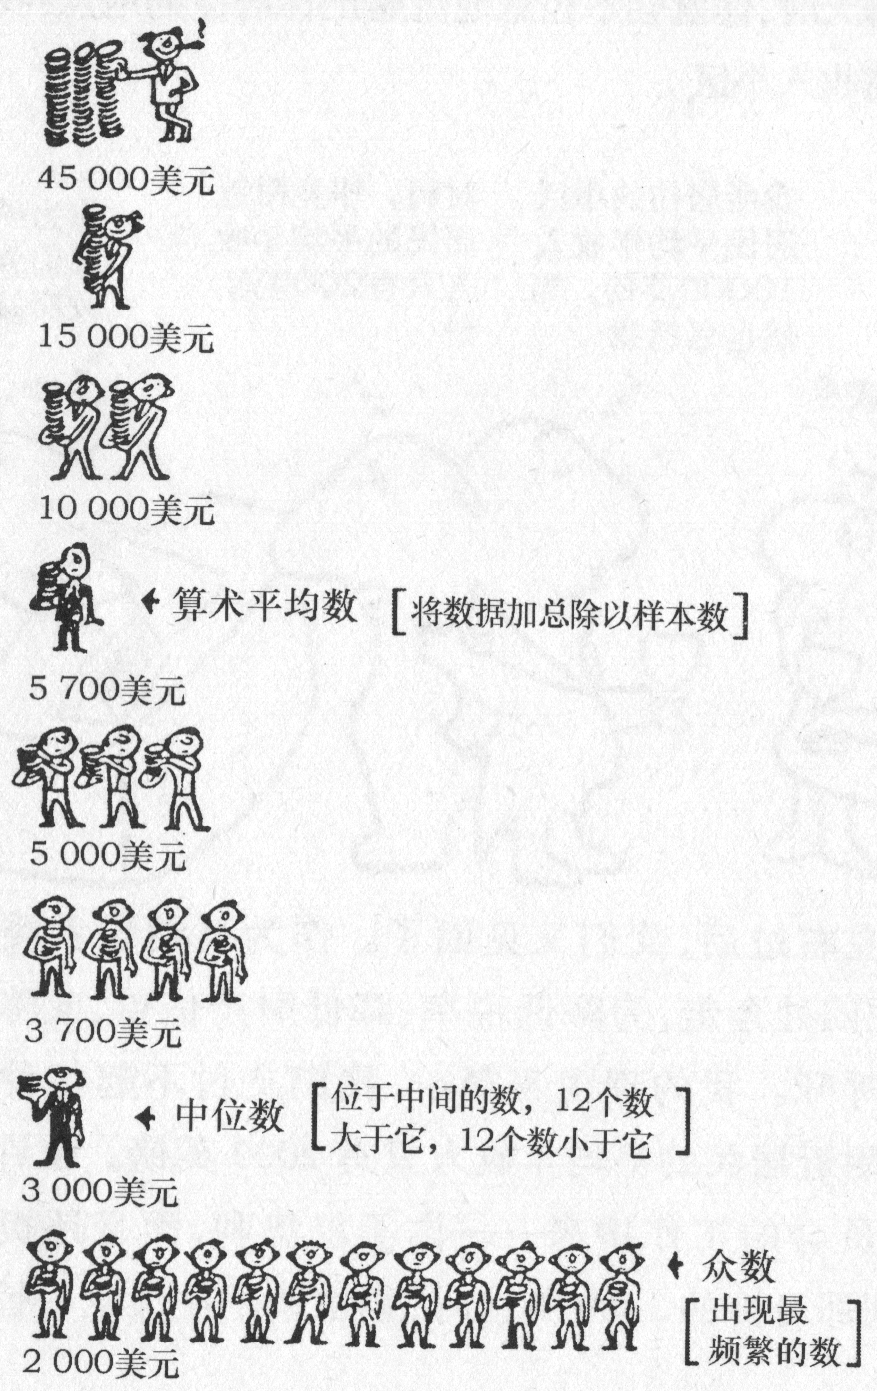
\includegraphics[width=0.4\textwidth]{c2.income.01.png}
  \end{figure}
\end{frame}

\begin{frame}
  \frametitle{案例 | 小区居民年收入 | 总结}
  \begin{block}{正态分布}
在处理诸如人类特征的数据时,各种平均数的数值十分接近。这些数据具有我们常说的正态分布的形态特点,在用曲线绘制正态分布时,将看到一条钟形的曲线,均值、中位数和众数都落在相同的点上。
  \end{block}
  \pause
  \begin{block}{非正态分布}
收入的分布不再像钟形一样对称,而是有偏的,它的形状类似于孩子玩的滑梯,梯子一侧是陡斜地升到顶部,而滑道一侧则缓慢向下倾斜。此时,均值与中位数、众数相差甚远。
  \end{block}
  \vspace{-0.5em}
  \begin{figure}
    \centering
    \visible<2->{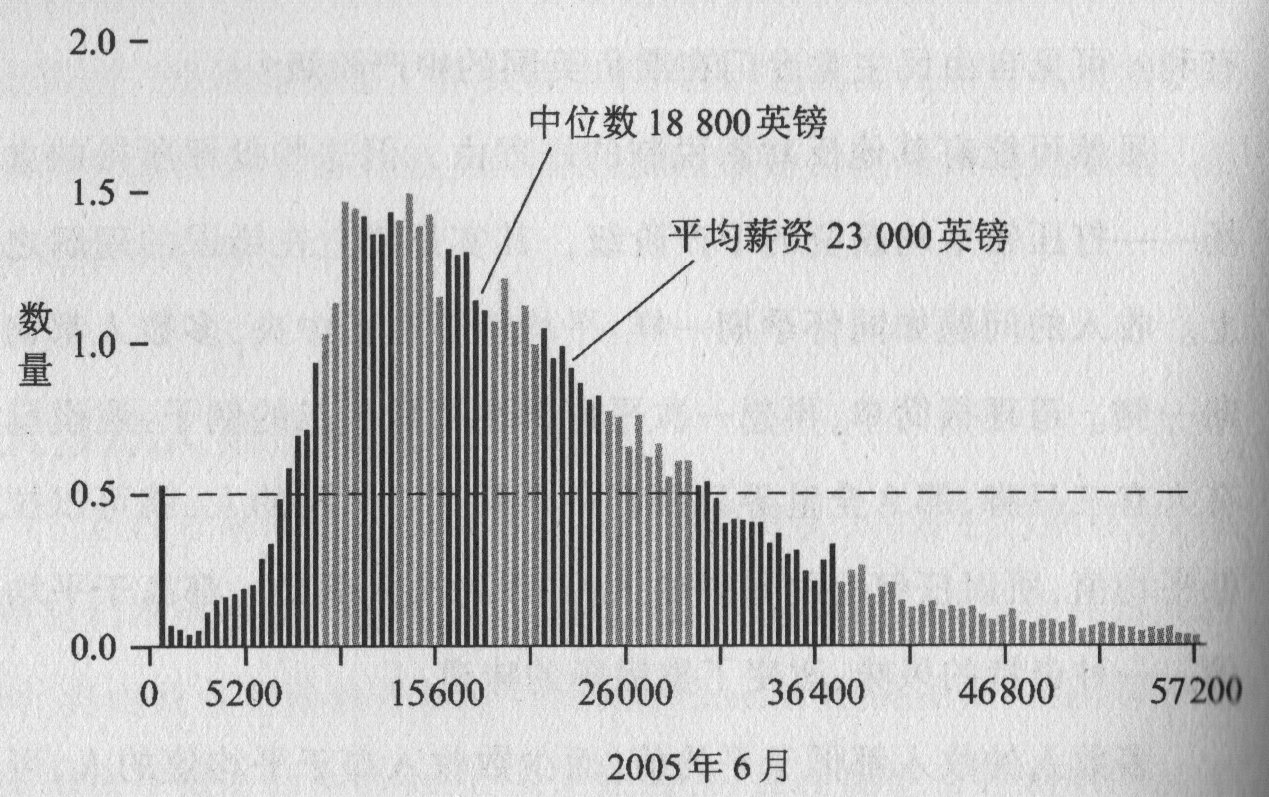
\includegraphics[width=0.4\textwidth]{c2.income.02.png}}\quad
    \visible<2->{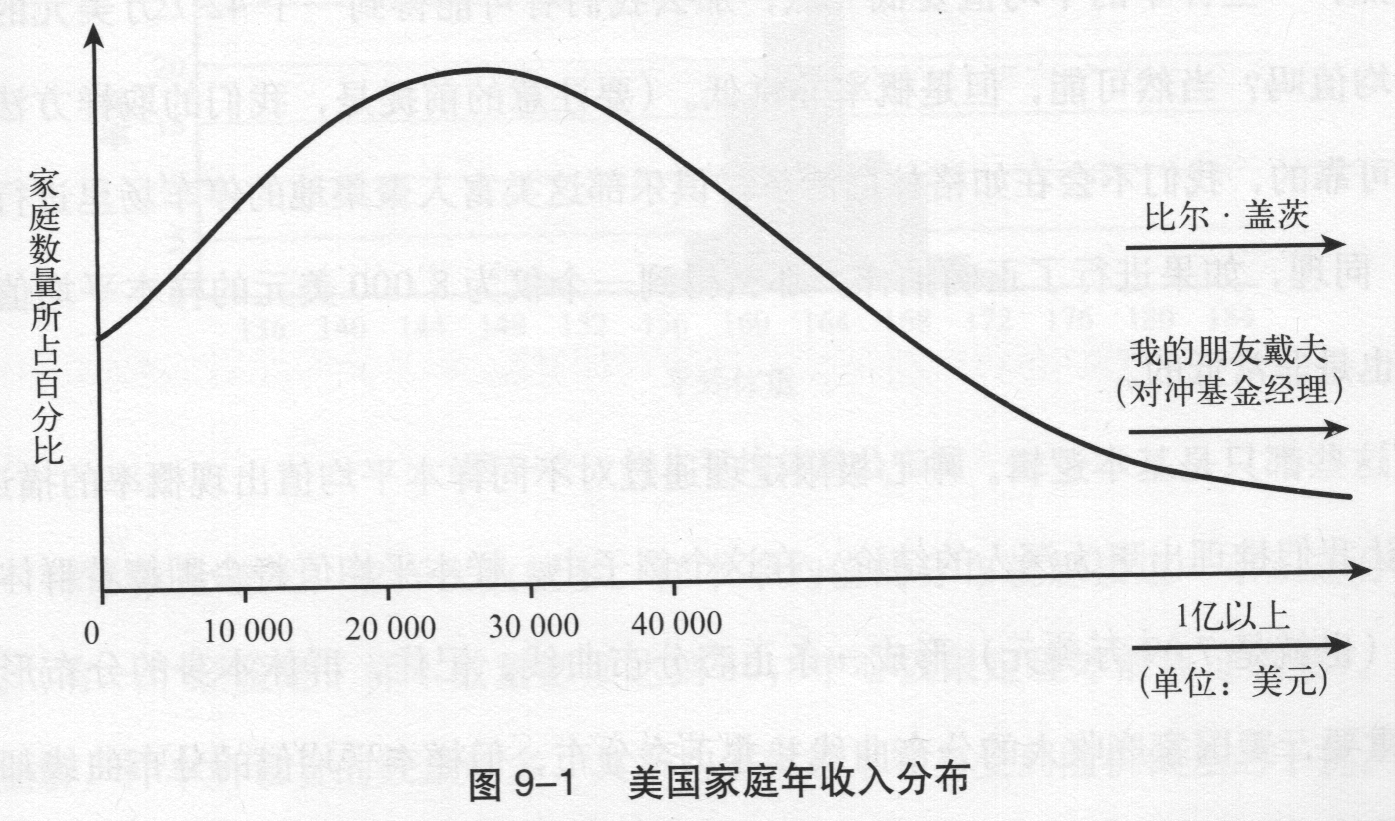
\includegraphics[width=0.43\textwidth]{c2.income.03.png}}
  \end{figure}
\end{frame}

\begin{frame}
  \frametitle{案例 | 小区居民年收入 | 总结}
  \begin{figure}
    \centering
    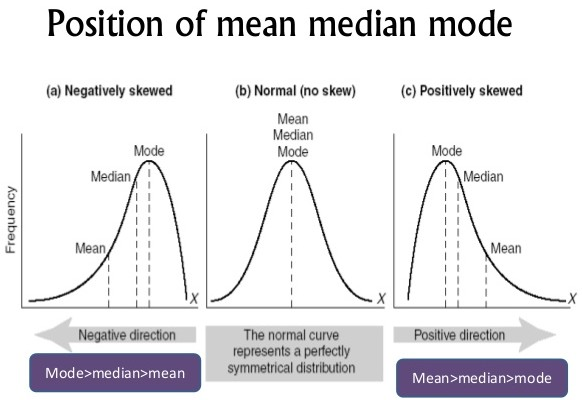
\includegraphics[width=0.85\textwidth]{c2.md.01.jpg}
  \end{figure}
\end{frame}

\begin{frame}
  \frametitle{案例 | 公司员工收入}
  \begin{block}{公司员工的平均收入}
    当你听到公司执行总裁或企业所有者宣称,在他的企业中员工的平均收入是多少时,你应该好好思考一下其中的原因。
    \begin{itemize}
      \item 如果这个数是中位数,你可以获得一些显而易见的信息:一半员工赚得比它多,一半比它少。
      \item 如果是均值(当没有确切指出它的种类时,多半是均值),它仅仅是所有者的高收入与全体工人低水平收入的平均数,根本没有什么意义。“平均年收入为3800英镑”既隐瞒了1400英镑的低收入,又隐瞒了所有者以巨额薪金形式抽取的高额利润。
    \end{itemize}
  \end{block}
\end{frame}

\begin{frame}
  \frametitle{案例 | 公司员工收入}
  \begin{figure}
    \centering
    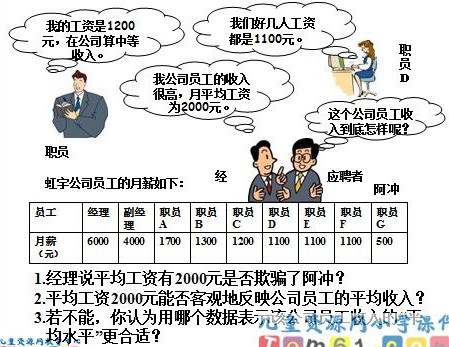
\includegraphics[width=0.8\textwidth]{c2.gongsi.01.jpg}
  \end{figure}
\end{frame}

\begin{frame}
  \frametitle{案例 | 公司员工收入 | 公司的声明}
  \begin{block}{背景介绍}
谭武是某个小型制造企业的3个合伙人之一。到了年底,谭武给企业的90个职工共发了99000英镑;谭武和其他合伙人每人各获得5500英镑的工资;最后还余下21000英镑,作为利润可供3个合伙人平分。谭武将如何说明这种情况呢?
  \end{block}
  \pause \pause \pause \pause
  \begin{block}{初级方案}
    为了便于理解,谭武打算采用平均数的形式:
    \begin{description}
      \item[职工的平均工资] 1100英镑($99000 / 90 = 1100$)
      \item[所有者的平均工资及利润] 12500英镑($((5500 x 3) + 21000) / 3 = 12500$)
    \end{description}
  \end{block}
  \pause
  \begin{block}{谭武的思考}
    这看上去太不公平了,自己都看不过去!
  \end{block}
\end{frame}

\begin{frame}
  \frametitle{案例 | 公司员工收入 | 公司的声明}
  \begin{block}{换一种形式}
    \begin{enumerate}
      \item 从21000英镑的利润中拿出15000英镑以奖金的形式平分给3位合伙人
      \item 将包括了所有者和职工的工资进行平均
    \end{enumerate}
  \end{block}
  \pause
  \begin{block}{改进方案}
    \begin{description}
      \item[所有人员的平均工资或薪金] 1403英镑($(99000 + 5500 x 3 + 15000) / 93 = 1403.226$)
      \item[所有者平均利润] 2000英镑($(21000 - 15000) / 3 = 2000$)
    \end{description}
  \end{block}
  \pause
  \begin{block}{谭武的思考}
    现在看上去好多了,足以作为公布的内容张贴在公告栏中,或者作为与职工谈判的依据。
  \end{block}
\end{frame}

\begin{frame}
  \frametitle{案例 | 公司员工收入 | 公司的声明}
  \begin{block}{总结}
    \begin{itemize}
      \item 本质不变:总的钱数没变,每个职工拿到的钱数没变,每个合伙人拿到的钱数没变!
      \item 表象反转:最终的结论/声明/公告竟有天壤之别!
    \end{itemize}
  \end{block}
  \pause
  \begin{block}{初级方案}
    \begin{description}
      \item[职工的平均工资] 1100英镑($99000 / 90 = 1100$)
      \item[所有者的平均工资及利润] 12500英镑($((5500 x 3) + 21000) / 3 = 12500$)
    \end{description}
  \end{block}
  \pause
  \begin{block}{改进方案}
    \begin{description}
      \item[所有人员的平均工资或薪金] 1403英镑($(99000 + 5500 x 3 + 15000) / 93 = 1403.226$)
      \item[所有者平均利润] 2000英镑($(21000 - 15000) / 3 = 2000$)
    \end{description}
  \end{block}
\end{frame}

\begin{frame}
  \frametitle{案例 | 收入}
  \begin{block}{收入}
    \begin{itemize}
      \item 收入的问题如同怀孕期一样:平均值不在正中央,多数人都偏向一侧。
      \item 多数人的收入都低于平均值,而少数收入高于平均值的人,将平均值远远拉离中间数。
      \item 因为平均收入被拉高了,以致多数人的收入都低于平均值。
      \item 领平均薪资的人已经算是相当富有了,因为平均值已经被少数高收入者远远拉离中间数。
      \item 从经济的角度而言,很多有关“英国中产阶级”的政治媒体言论根本不晓得“中产阶级”的定义是什么。
    \end{itemize}
  \end{block}
\end{frame}

\begin{frame}
  \frametitle{案例 | 收入}
  \begin{block}{有钱的巨人}
  \begin{figure}
    \centering
    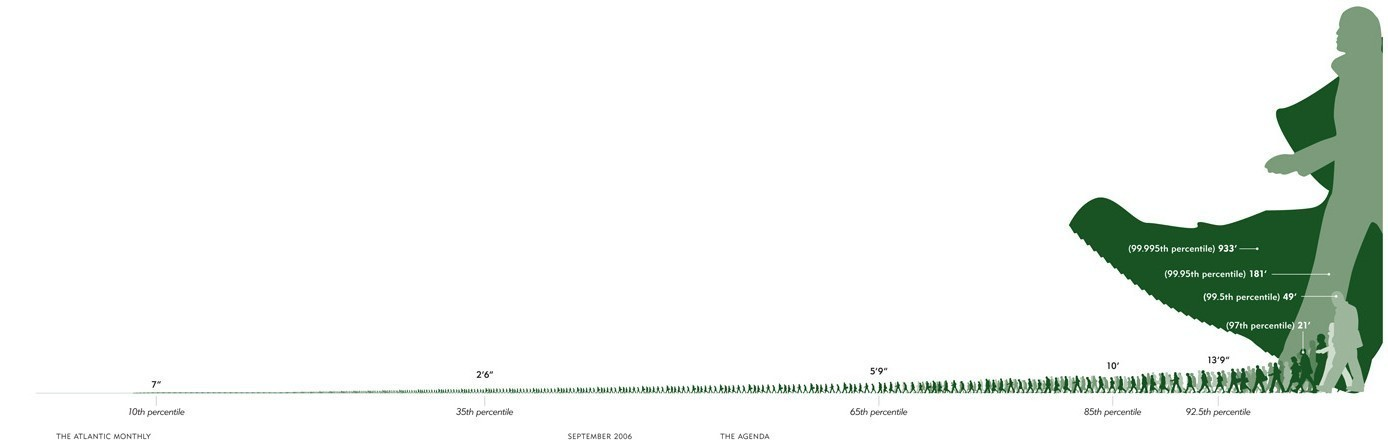
\includegraphics[width=\textwidth]{c2.money.01.jpg}
  \end{figure}
  一个百万富翁对于平均值的影响,远大于成千上万个贫民,而亿万富翁的影响力则又大了100倍。他们的影响力,大到让全世界80\%人口的财富低于平均值。
  \end{block}
\end{frame}

\begin{frame}
  \frametitle{案例 | 收入}
  \begin{block}{总结}
    当你看到某个平均收入时,首先问问:是什么的平均?包括了哪些人?
  \end{block}
  \pause
  \begin{block}{包括了哪些人?}
    美国钢铁公司曾经指出:10年间,该公司职工的平均周收入攀升了107\%!然并卵……
    \pause
    \begin{itemize}
      \item 早期的数据包括了兼职员工
      \item 如果你某年只工作了半年,而第二年全年都在工作,你的收入毫无疑问会翻番,但这并不意味着工资率发生了变动。
    \end{itemize}
  \end{block}
\end{frame}

\begin{frame}
  \frametitle{案例 | 收入}
  \begin{block}{报道}
    你也许曾在报纸上看到过,某年美国的家庭平均收入是6940美元。别太在意这个数字,除非知道:
    \begin{itemize}
      \item 这个数字包括了哪些家庭?
      \item 使用了哪种平均数?
      \item 谁说的?他是如何获得该信息的?这个数的准确性如何?
    \end{itemize}
  \end{block}
  \pause
  \begin{block}{普查局}
    \begin{itemize}
      \item “家庭”是指两个或更多具有亲属关系的人住在一起所形成的“家庭”。
      \item 这是个中位数。
      \item 数据建立在抽样基础上,该调查以19/20的概率保证真实的数值会落在估计值加减71美元的范围之内。
    \end{itemize}
  \end{block}
\end{frame}

\begin{frame}
  \frametitle{案例 | 中产阶级}
  \begin{block}{问题}
    美国中产阶级的经济健康状况如何?我们称之为“中产阶级”的人到底是更富了、更穷了,还是在原地踏步?
  \end{block}
  \pause
  \begin{block}{答案}
    一个合理的答案——肯定不会有“正确”的答案——就是,计算一代美国人(大约为30年)的人均收入,观察其变化趋势。
  \end{block}
  \pause
  \begin{block}{存在的问题}
    \begin{itemize}
      \item 没有考虑通货膨胀因素
      \item 我们需要知道的是普通美国人的收入,而不是泛泛的人均收入,这两者有本质上的区别
    \end{itemize}
  \end{block}
\end{frame}

\begin{frame}
  \frametitle{案例 | 中产阶级 | 通货膨胀}
  \begin{figure}
    \centering
    \visible<1->{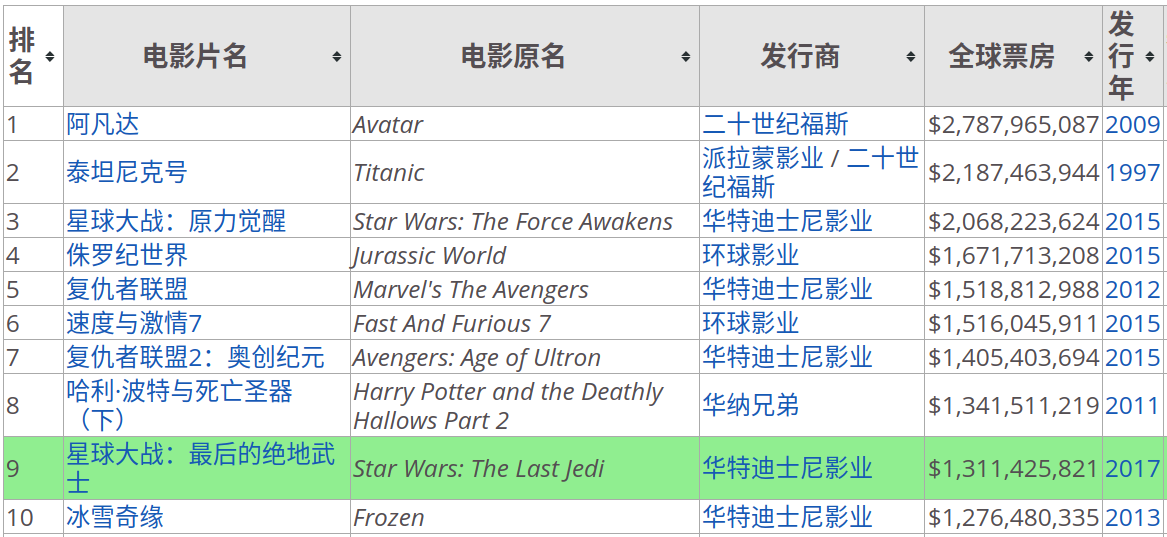
\includegraphics[width=0.78\textwidth]{c2.movie.01.png}}\\
    \visible<2->{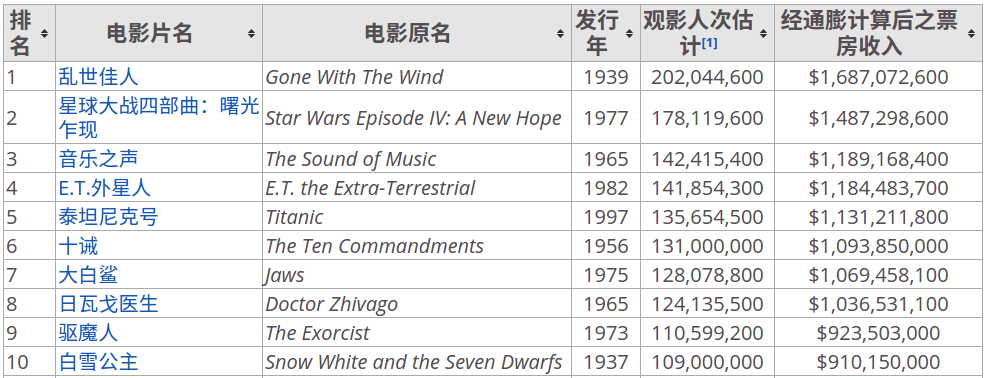
\includegraphics[width=0.78\textwidth]{c2.movie.02.png}}
  \end{figure}
\end{frame}

\begin{frame}
  \frametitle{案例 | 中产阶级 | 通货膨胀}
  \begin{figure}
    \centering
    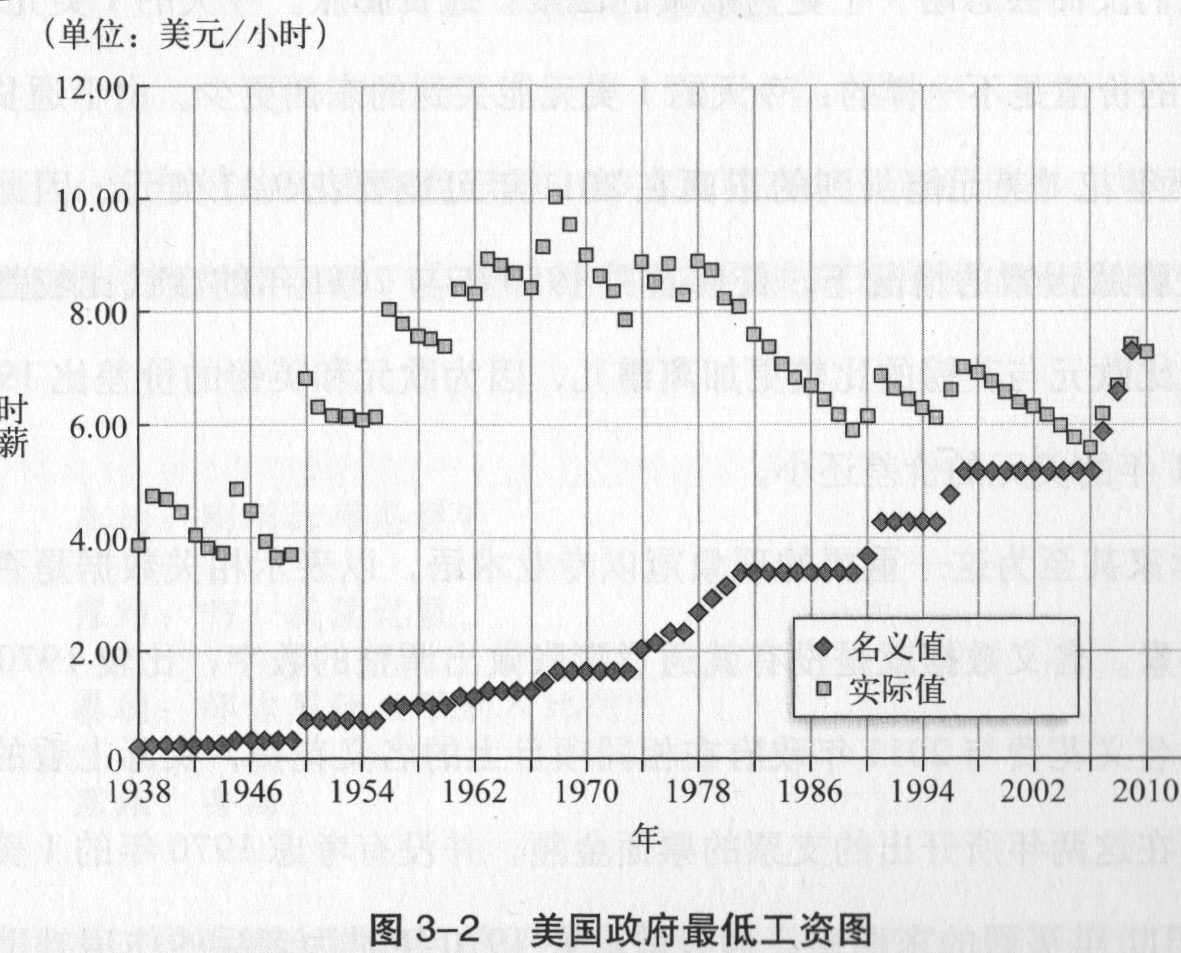
\includegraphics[width=0.8\textwidth]{c2.coin.01.png}
  \end{figure}
\end{frame}

\begin{frame}
  \frametitle{案例 | 中产阶级}
  \begin{block}{专家的答案}
    要评价美国“中产阶级”的经济状况,我们需要了解(通货膨胀调整后的)工资中位数在过去几十年中的变化,还建议留意一下处于第25百分位数和第75百分位数人群的工资变化,因为这两拨人通常被认为是中产阶级中的高收入和低收入人群。
  \end{block}
  \pause
  \begin{block}{注意}
    在评价经济状况的过程中,不能将收入和工资等同起来。这两者是不同的,工资是我们付出的固定份额的劳动所得,如时薪或周薪;收入是全部所得的总和,来源有多种。相比于收入来说,工资是评价美国人劳动收益的一个更加直观的指标,工资越高,工人们每工作1小时能领到的钱也就越多。
  \end{block}
\end{frame}

\begin{frame}
  \frametitle{案例 | 中产阶级}
  \begin{figure}
    \centering
    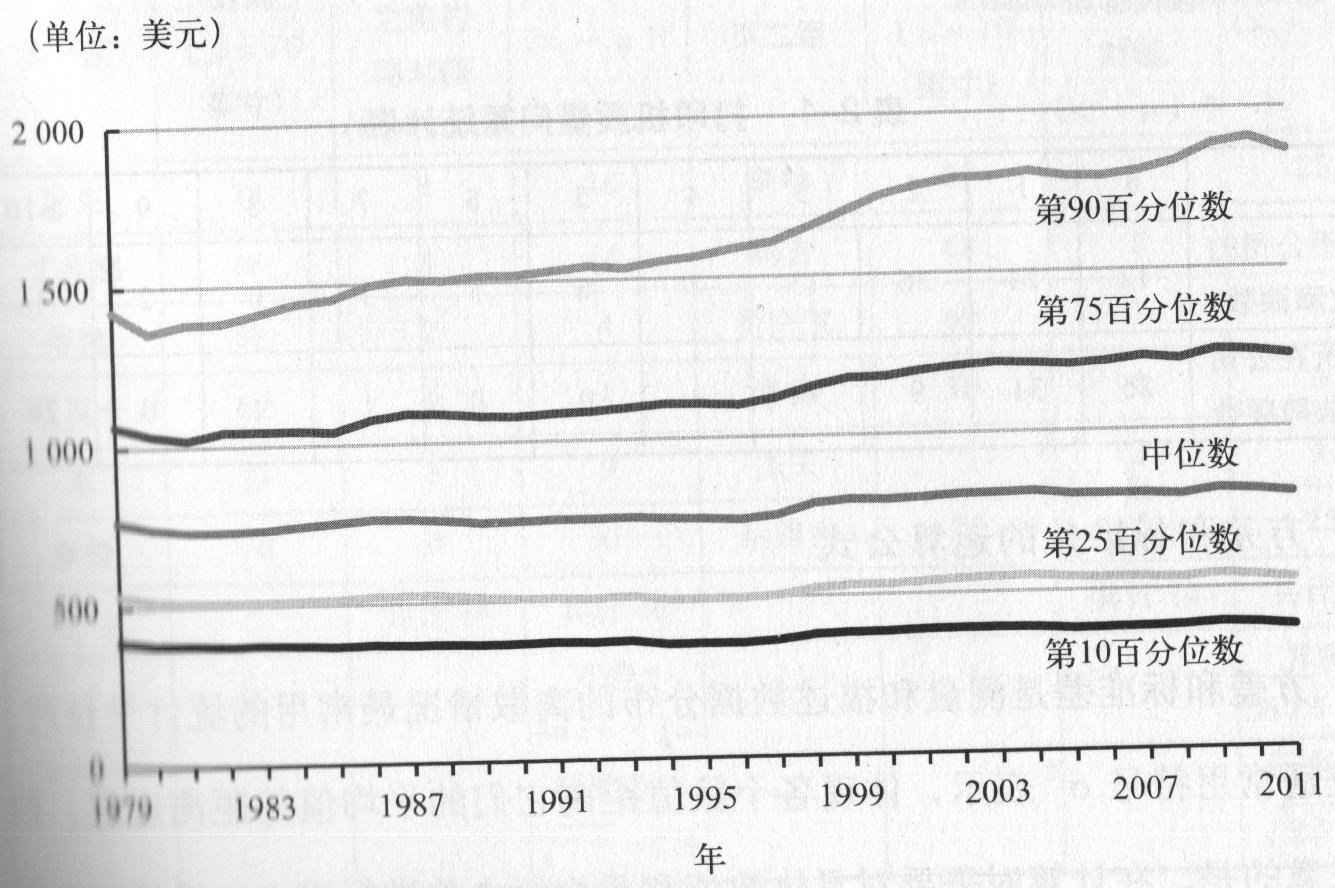
\includegraphics[width=0.9\textwidth]{c2.usa.01.png}
  \end{figure}
\end{frame}

\begin{frame}
  \frametitle{案例 | 减税政策}
  \begin{block}{减税政策}
    美国前总统小布什政府的说法,减税政策将惠及绝大多数的美国家庭。在这项政策推行后,将会有9200万美国人享受减税待遇,人均减税额超过1000美元(具体数字应该是1083美元)。这个关于减税政策的概括准确吗?
  \end{block}
  \pause \pause \pause \pause
  \begin{block}{解析}
    《纽约时报》评价说:“数据本身并没有撒谎,只不过有些数据没有发出声音罢了。”是不是会有9200万美国人将享受减税待遇?答案是肯定的。那么,这些人中的大部分人都可以少缴纳约1000美元的税款吗?不是的。因为减税额的中位数还不足100美元。只有数量相对少的巨富们才有资格享受大额减税,而正是这些人拉高了平均值,让人均减税额看起来比绝大多数美国人真正享受到的要高。
  \end{block}
\end{frame}

\section{其他案例分析}
\begin{frame}
  \frametitle{案例 | 跳绳成绩}
  \begin{figure}
    \centering
    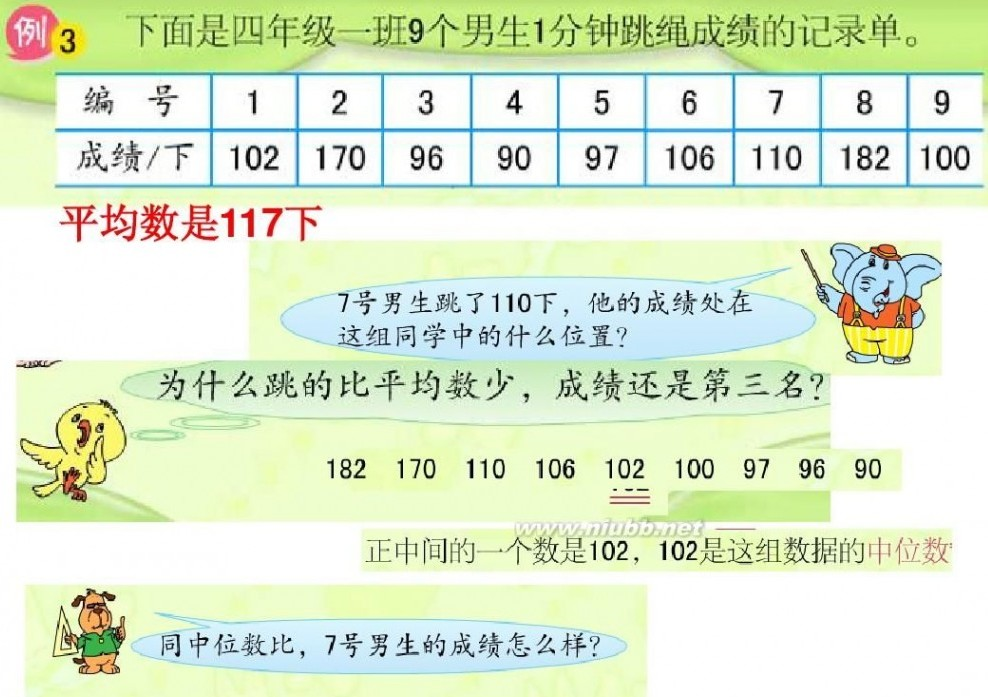
\includegraphics[width=0.9\textwidth]{c2.tiaosheng.01.jpg}
  \end{figure}
\end{frame}

\begin{frame}
  \frametitle{案例 | 小新的成绩}
  \begin{figure}
    \centering
    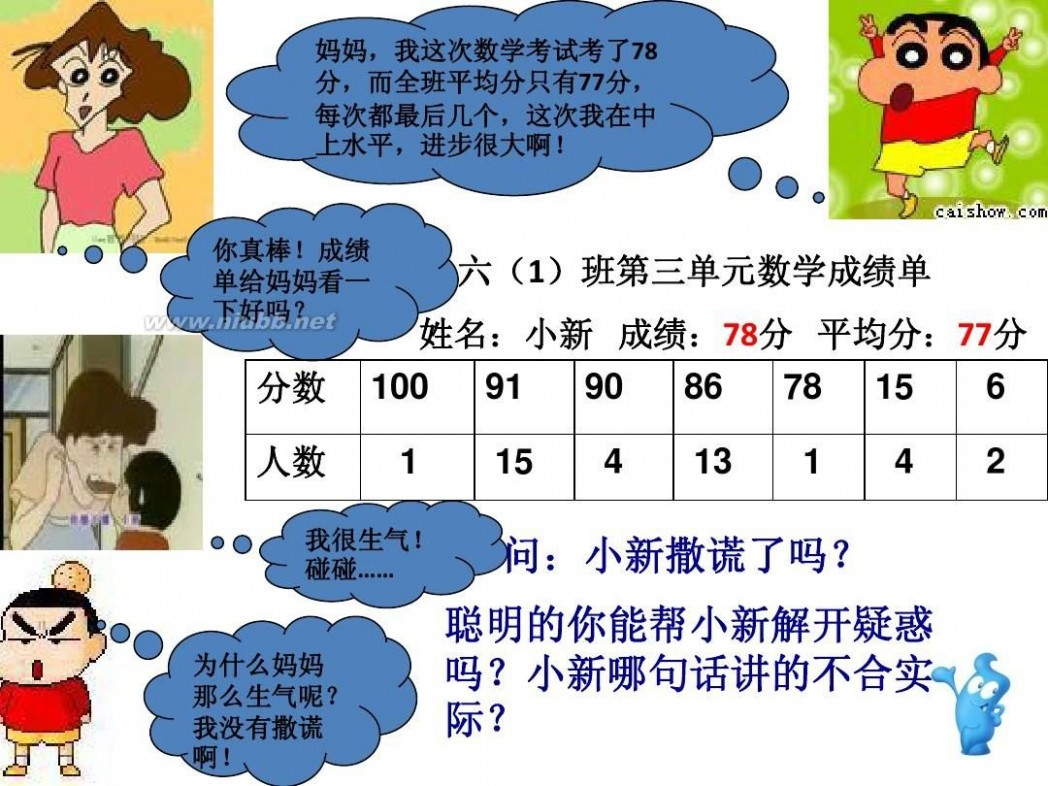
\includegraphics[width=0.8\textwidth]{c2.xiaoxin.01.jpg}
  \end{figure}
\end{frame}

\begin{frame}
  \frametitle{案例 | 其他}
  \begin{block}{其他}
    \begin{itemize}
      \item 我们每个人的脚,几乎都比平均脚数多。
      \item ……
    \end{itemize}
  \end{block}
\end{frame}

\begin{frame}
  \frametitle{案例 | 统计 vs. 战术 vs. 谎言}
  \begin{figure}
    \centering
    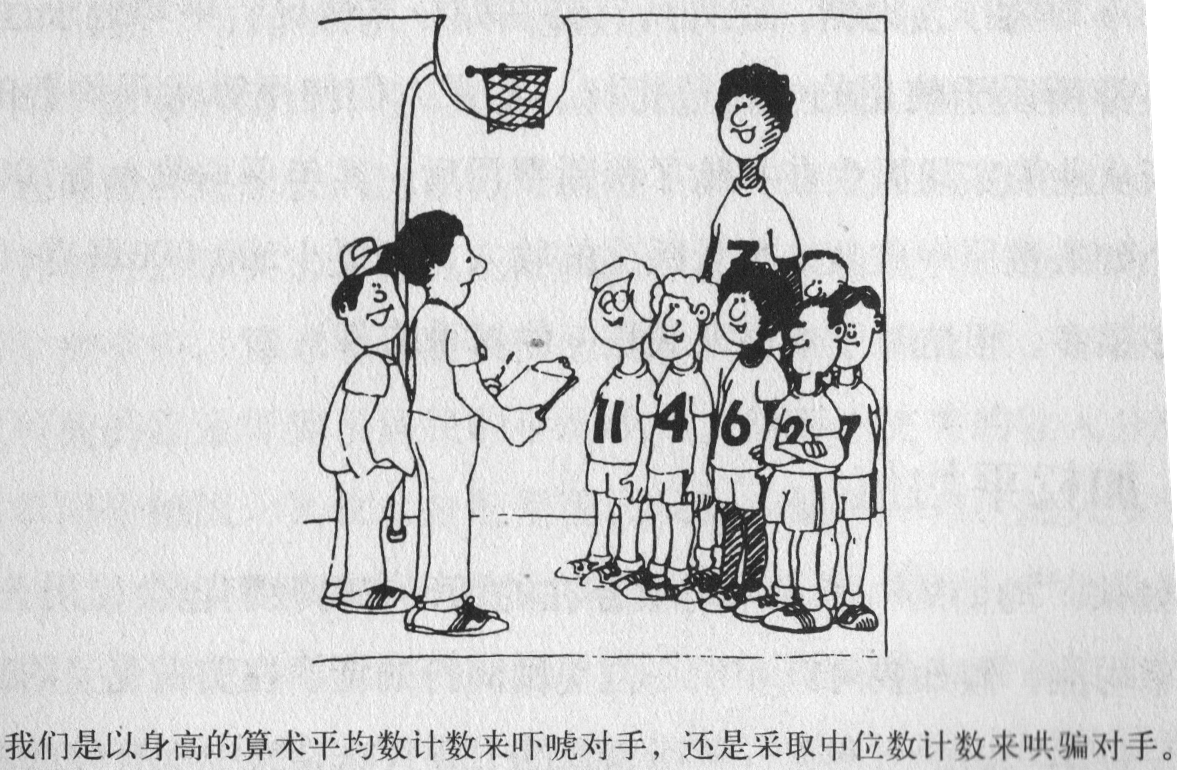
\includegraphics[width=0.9\textwidth]{c2.height.01.png}
  \end{figure}
\end{frame}

\begin{frame}
  \frametitle{案例 | 《时代》杂志的订户}
  \begin{block}{“编者的话”}
    \begin{description}
      \item[旧订户] 年龄的中位数是41岁,家庭平均年收入为9535美元。
      \item[新订户] 年龄的中位数是34岁,家庭平均年收入为7270美元。
    \end{description}
  \end{block}
  \pause
  \begin{block}{疑问}
    为什么两次谈到年龄时都指出采用了中位数,而关于收入却不明确平均数的类型?
  \end{block}
  \pause
  \begin{block}{猜想}
    也许收入使用的是数值较大的均值,以达到利用高收入读者群吸引广告商的目的。
  \end{block}
\end{frame}

\begin{frame}
  \frametitle{案例 | 平均寿命}
  \begin{figure}
    \centering
    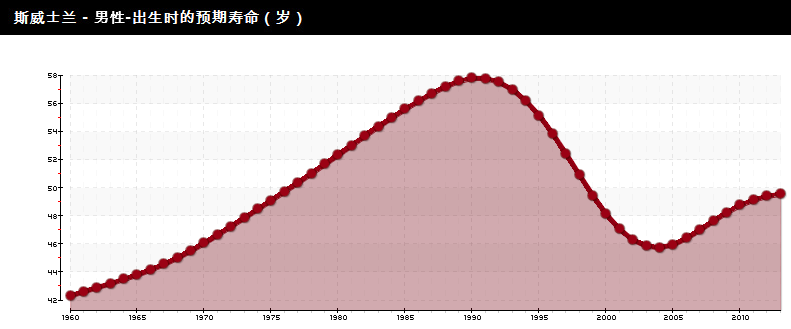
\includegraphics[width=0.48\textwidth]{c2.swsl.man.01.png}
    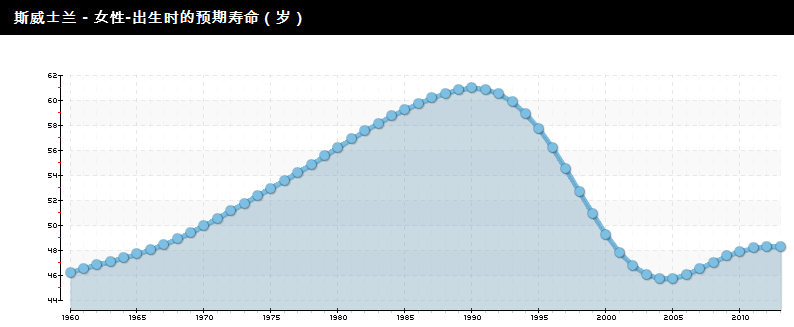
\includegraphics[width=0.48\textwidth]{c2.swsl.woman.01.png}
  \end{figure}
  \vspace{-1em}
  \begin{block}{可怜的斯威士兰人?}
    斯威士兰人的平均寿命低得吓人,男性为32岁,女性为33岁(32岁并不是一个常见的死亡年龄,大多数活过32岁的人都可以活得更久)
  \end{block}
  \pause \pause \pause \pause
  \begin{block}{夭折的婴儿!}
    为了要计算平均值,他们与因为缺乏医疗资源而夭折的婴儿并在一起计算,而这些早逝天使的数量又很多,于是斯威士兰人的平均寿命就被婴儿的高死亡率拉低。
  \end{block}
\end{frame}

\begin{frame}
  \frametitle{案例 | 平均寿命}
  \begin{figure}
    \centering
    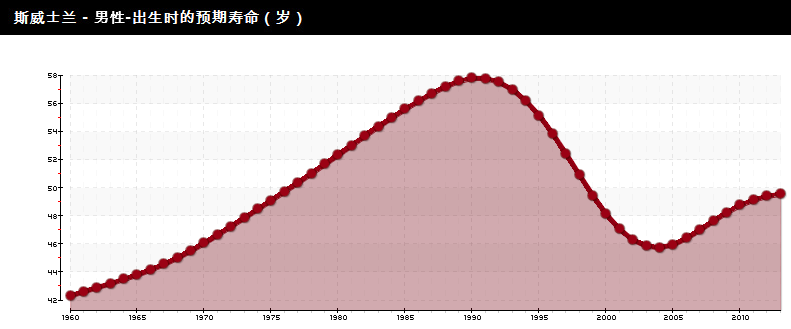
\includegraphics[width=0.48\textwidth]{c2.swsl.man.01.png}
    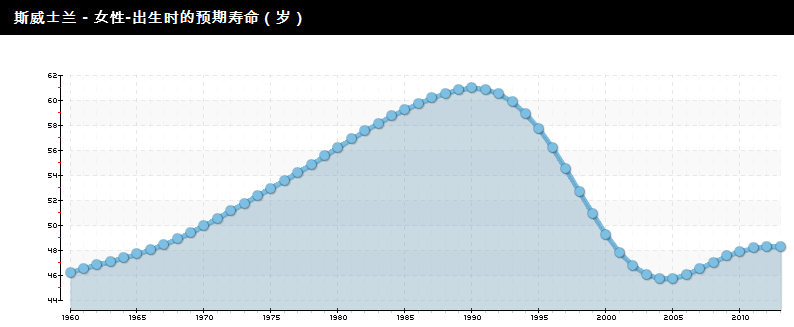
\includegraphics[width=0.48\textwidth]{c2.swsl.woman.01.png}\\
    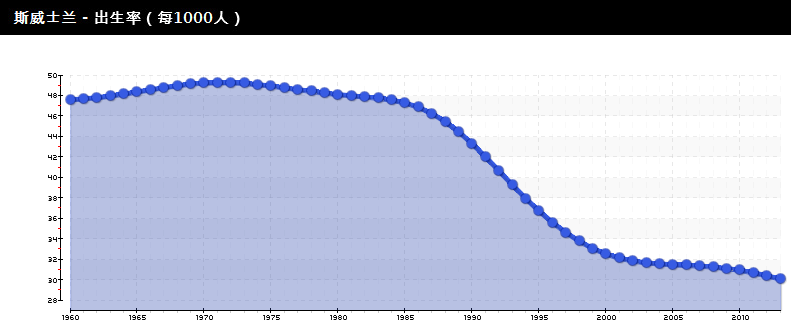
\includegraphics[width=0.48\textwidth]{c2.swsl.baby.birth.01.png}
    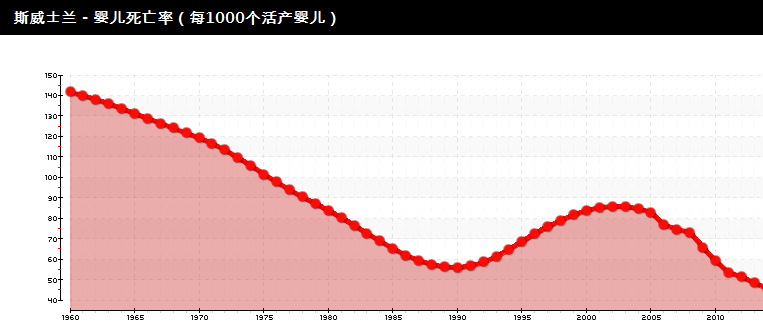
\includegraphics[width=0.48\textwidth]{c2.swsl.baby.death.01.png}\\
  \end{figure}
\end{frame}

\begin{frame}
  \frametitle{案例 | 癌症存活率的真相}
  \begin{block}{引言}
    事物实际上通常呈现两极化,但平均值把这两极拉在一起。
  \end{block}
  \pause
  \begin{block}{癌症存活率}
    \begin{itemize}
      \item 古尔德,腹部间皮癌
      \item 存活时间的中位数只有8个月:有一半的患者活不过8个月,另一半的人可以活得更久
      \item 存活时间的排行,在中位数右方的曲线,有一条延伸数年的尾巴
      \item 存活了20年(因为另一种不相关的癌症而去世)
    \end{itemize}
  \end{block}
\end{frame}

\begin{frame}
  \frametitle{案例 | 预产期为什么都不准?}
  \begin{block}{预产期}
    从最后一次月经来潮的第一天开始,往后推算280天(平均值)。
  \end{block}
  \pause
  \pause
  \pause
  \begin{block}{预产期不准确的原因}
    \begin{itemize}
      \item 有些孕妇会早产
      \item 几乎没有孕妇可以过了预产期两周以上,而医生还不实施人工催生
    \end{itemize}
早产会让怀孕期的平均值下降,延迟则会拉高平均值的天数,但我们用人为的力量介入,阻止宝宝晚于平均值两周以上出生。这种只计算每个早产儿却排除晚生的宝宝所造成的不平衡效果,会使怀孕期的平均值低于自然的天数。
  \end{block}
  \pause
  \begin{block}{280天理论的轮回}
    我们的行为以平均值作为依据,但这个数字之所以会变成平均值,却是我们的行为所造成的。
  \end{block}
\end{frame}

\begin{frame}
  \frametitle{案例 | 预产期为什么都不准?}
  \begin{block}{总结}
    合并过早与过晚两个极端边界值的结果,产生了不准确的预产期。
  \end{block}
  \pause
  \begin{block}{大规模研究}
    40万名的瑞典妇女,大部分的准妈妈们都超过280天还没生产。到了第282天(中位数),有一半的婴儿已经出生;但人数最多的怀孕期,也是最能够当做每个人可能的怀孕期,是283天(众数)。
  \end{block}
  \pause
  \begin{block}{结论}
    近期研究证实的数据:最常见也最可能的怀孕期是283天。
  \end{block}
\end{frame}

\section{安全的旅行方式}
\begin{frame}
  \frametitle{案例 | 安全的旅行方式}
  \begin{block}{问题}
    人们在路上旅行时究竟采用哪一种方式更加安全,是乘坐飞机还是乘坐火车?(我们从一开始就把汽车看做是头号杀手。)
  \end{block}
  \pause
  \begin{block}{新闻报道}
    新闻媒体的报道好像乘坐飞机是一件十分可怕的事情。其实,飞行安全与否与我们是否经常翻阅报纸和杂志并没有直接的联系。
  \end{block}
\end{frame}

\begin{frame}
  \frametitle{案例 | 安全的旅行方式 | 飞机更安全}
  \begin{block}{飞机更安全}
    从平均意义上来看,也就是从基本的证据来看,可以说乘坐飞机旅行而遇难的人的确比乘坐火车遇难的人少。
  \end{block}
  \pause
  \begin{block}{统计数据}
    每100亿乘客公里数:
    \begin{description}
      \item[火车] 9人遇难
      \item[飞机] 3人遇难
    \end{description}
  \end{block}
  \pause
  \begin{block}{疑问}
    \begin{itemize}
      \item 如果这种统计数据正确,那么,乘坐火车旅行而遇难的人将会是乘坐飞机旅行遇难人数的3倍?
      \item 可是为什么当我们登上飞机的时候会出冷汗,而在乘坐火车时却不会这样?
    \end{itemize}
  \end{block}
\end{frame}

\begin{frame}
  \frametitle{案例 | 安全的旅行方式 | 火车更安全}
  \begin{block}{理性思考}
    从理性的角度出发,感兴趣的不是下一个千公里会遇难的可能性,而是在下一个小时内是否会遇难。
  \end{block}
  \pause
  \begin{block}{统计数据}
    每1亿乘客小时数:
    \begin{description}
      \item[火车] 7人遇难
      \item[飞机] 24人遇难
    \end{description}
  \end{block}
  \pause
  \begin{block}{结论}
    乘坐飞机旅行每小时所产生的死亡事故是乘坐火车旅行的3倍以上。
  \end{block}
\end{frame}

\begin{frame}
  \frametitle{案例 | 安全的旅行方式 | 总结}
  \begin{figure}
    \centering
    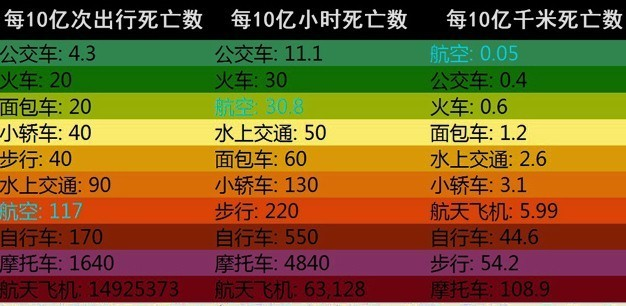
\includegraphics[width=0.9\textwidth]{c2.travel.01.jpg}
  \end{figure}
\end{frame}

\section{知识拓展}
\begin{frame}
  \frametitle{本福特定律}
  \begin{block}{本福特定律}
本福特定律,也称为本福特法则,说明一堆从实际生活得出的数据中,以1为首位数字的数的出现概率约为总数的三成,接近直觉得出之期望值1/9的3倍。推广来说,越大的数,以它为首几位的数出现的概率就越低。它可用于检查各种数据是否有造假。
  \end{block}
  \pause
  \begin{block}{应用}
    \begin{itemize}
      \item 1972年,Hal Varian提出这个定律来用作检查支持某些公共计划的经济数据是否有欺瞒之处。
      \item 1992年,Mark J. Nigrini提出以它检查是否有伪帐。
      \item 推而广之,它能用于在会计、金融甚至选举中出现的数据,应用于欺骗检测和股票市场分析等领域。
    \end{itemize}
  \end{block}
\end{frame}

\begin{frame}
  \frametitle{本福特定律}
  \begin{figure}
    \centering
    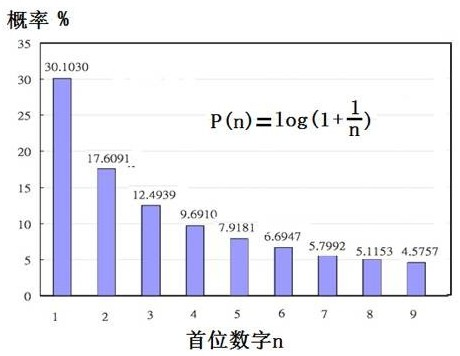
\includegraphics[width=0.4\textwidth]{c2.benford.01.jpg}\\
    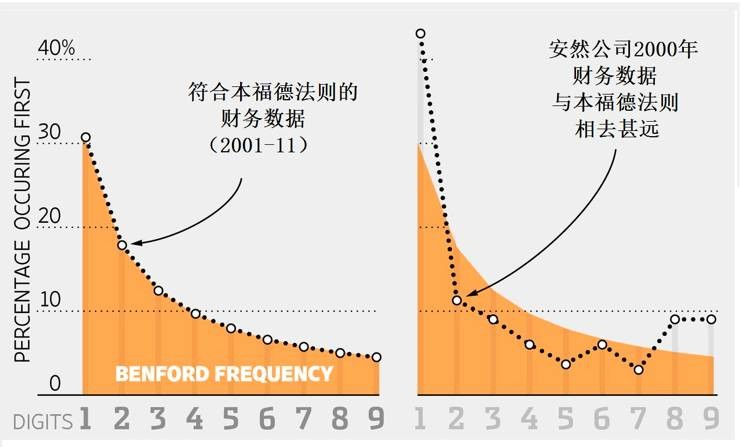
\includegraphics[width=0.6\textwidth]{c2.benford.02.jpg}
  \end{figure}
\end{frame}

\begin{frame}
  \frametitle{本福特定律}
  \begin{figure}
    \centering
    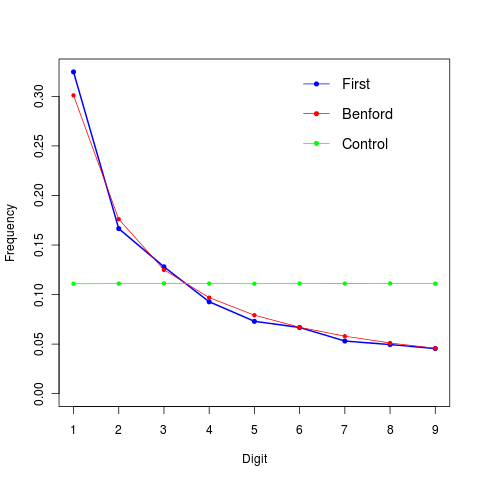
\includegraphics[width=0.48\textwidth]{c2.benford.03.png}
    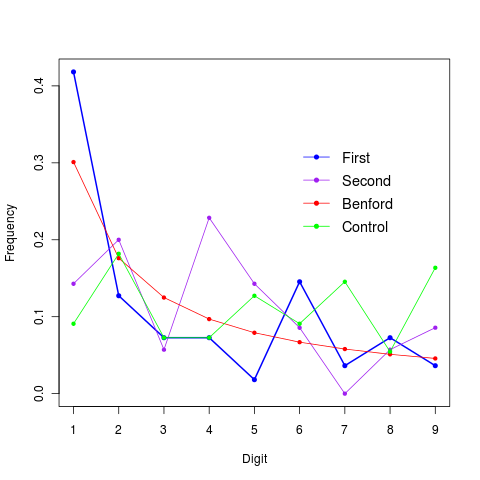
\includegraphics[width=0.48\textwidth]{c2.benford.04.png}
  \end{figure}
\end{frame}

\section{图说天下}
\begin{frame}
  \frametitle{图说天下}
  \begin{figure}
    \centering
    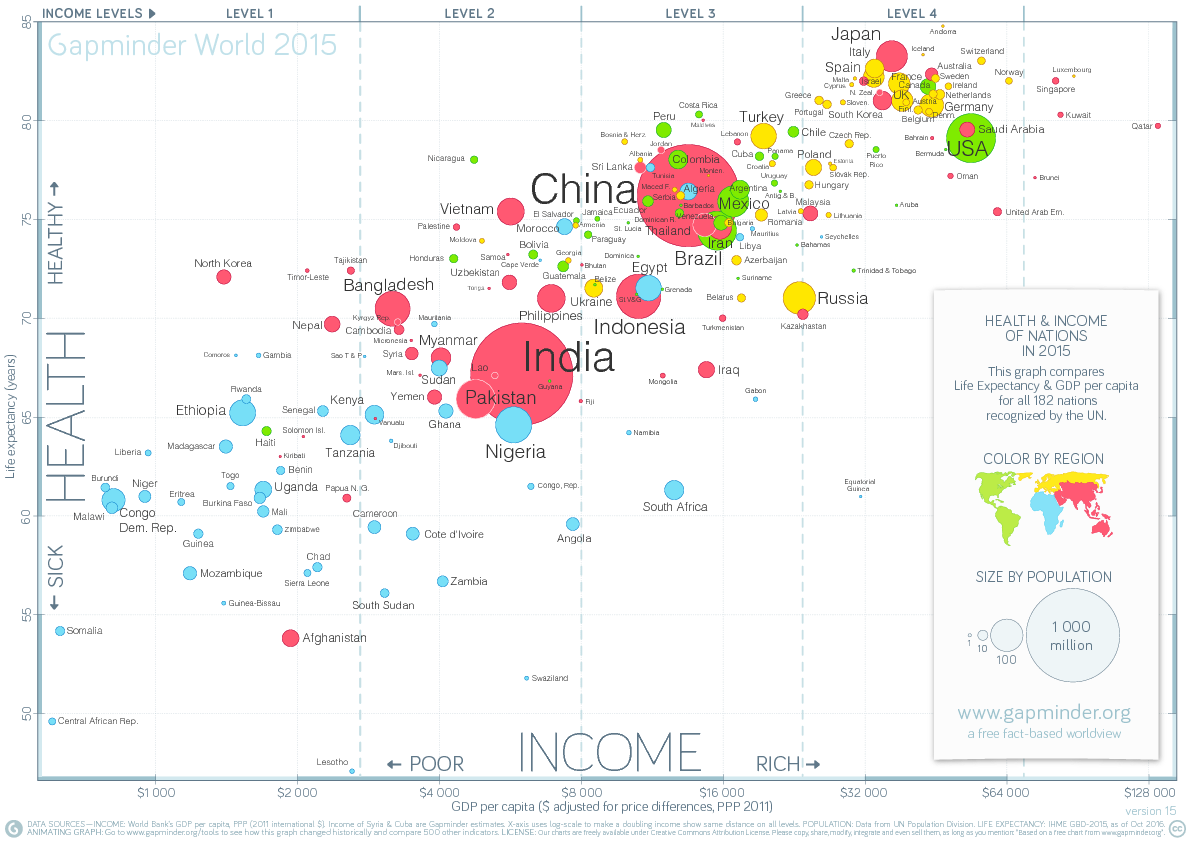
\includegraphics[width=0.9\textwidth]{c2.gapminder.2016.png}
  \end{figure}
  % \begin{itemize}
  %   \item \href{http://www.gapminder.org/downloads/updated-gapminder-world-poster-2015/}{http://www.gapminder.org/downloads/updated-gapminder-world-poster-2015/}
  %   \item \href{https://www.gapminder.org/tools}{https://www.gapminder.org/tools}
  % \end{itemize}
\end{frame}

\section{统计知识}
\begin{frame}
  \frametitle{总结}
  \begin{itemize}
    \item 平均值的优点在于,它缩小了庞大的信息量,让人得以管理惊人的数字,但也因为这个原因,使得它容易产生误导作用,让人忘记数字的差异性。平均值将所有的失误融为一体,这是它有用的地方,也是它骗人的地方。
    \item 当你被告知某个数是平均数时,除非能说出它的具体种类——均值,中位数,还是众数,否则你对它的具体涵义仍知之甚少。
    \item 在处理诸如人类特征的数据时,各种平均数的数值十分接近。这些数据具有正态分布的形态特点。
    \item 当你看到某个平均收入时,首先问问:是什么样的平均?包括了哪些人?
    % \item 类似的概率和误差范围构成了一个很好的估计。
    \item 遇到平均值时,要记得问:我们真正感兴趣的,是哪一个群体?在问平均薪资时,也许我们不会想知道金字塔顶端的人收入有多少,只想了解普通人的状况。
    \item 平均值是一个概略,有用,但所有的概略都是一个样。如果你不知道它只是个摘要,就会被它误导。平均值——是什么东西的平均值?请记得现实世界的多样性,别忘了彩虹原本是白色的。
  \end{itemize}
\end{frame}

\begin{frame}
  \frametitle{总结}
  \begin{block}{平均值 vs. 世界的多样化}
    \begin{itemize}
      \item 平均值只能够说个大概,这是它们天生的说话方式。用这么简单的方式来描述一个群体,重要的细节无可避免就会被含糊带过。平均值就像晚间新闻的一句结语,简单地说出记者所归纳的重点,但是没看过报道的观众,还是不知道具体的新闻内容是什么。它向来有个问题,宣称自己为这个万花筒般的世界发声,却扼杀了我们所有的想象。想要看穿平均值的真面目,首先你得记得世界的多样化。
      \item 平均薪资、平均房价、平均寿命、平均犯罪率,这些以平均为首的名词,以及其他同等性质的平均数,如通货膨胀率等,全都把数字单一化,将一堆数据总结成一个代表总体的数字或是图上的一点。平均值既有优点,也有缺点,它铲平山丘、填满坑谷,让我们误以为地球真的是平的。事实上,地球是起伏不平的。
      \item 彩虹原本是白色的,经过折射和反射之后,白色的太阳光线变成了神奇的七彩颜色。每当你看见平均值时,请想起“彩虹是白色的”这句话,并想象经过折射、反射出现的七彩霓虹。
    \end{itemize}
  \end{block}
\end{frame}




\section*{Acknowledgements}
\begin{frame}
  \frametitle{Powered by}
  \begin{center}
    
\includegraphics[width=9cm]{power.png}
  \end{center}
\end{frame}

\end{document}

